\section{Methodology}

The primary aim of this study was to understand how the values and motivations of the three design partners---\NGO{}, \PC{} and the research team---were reflected in the design of the IVR system, and shaped by the constraints and possibilities that it offered. Design ethnography is a research approach that draws influence from both ethnography and design: providing a critical and reflexive lens to a design process, and providing insight into how the entanglement of actors, artefacts and processes within a context shapes design decisions and outcomes \cite{akama2015, smith2016}. In this study, the design ethnography was carried out by a researcher who was working alongside (but independently to) the researchers co-designing the IVR system with \NGO{} and \PC{}. 

Design workshops were carried out online over 11 months (November 2020 - September 2021) as \PC{} and \NGO{} were situated in Dhaka, Bangladesh, whilst the researchers were situated in Melbourne, Australia. Travel between these two locations was not possible due to travel restrictions imposed by the Australian government in response to the COVID-19 global pandemic. Research activities involved 12 x 1h online video conferencing design workshops, with at least one researcher and one representative of \PC{}. An \NGO{} representative was present at 8 of these online workshops. 

These workshops were carried out over three design phases: 
\begin{enumerate}
\item \textit{Exploratory discussions}, which aimed to understand the various partners and their priorities in this process. In these workshops, each stakeholder shared their specific interest in the process, their motivations for participating, and their intended outcomes. During this stage \PC{} shared further details about their services, business model, structure and challenges and their underlying motivations for the design and use of this IVR system; whilst \NGO{} provided details of the plight of domestic workers they have been supporting through their advocacy work, and their ideas of how the platform could improve the workers' livelihoods (e.g. through financial security and personal safety). 

\item \textit{Iterative design}, which aimed to develop an initial iteration of the IVR flow that reflected the needs and priorities of \PC{} and \NGO{}. \PC{} led this phase, producing several iterations of the IVR system design in Microsoft PowerPoint detailing the `IVR flow': the menus, information and options available to the domestic workers as they interact with the system over the phone (Figure \ref{fig:ivrFlow}). During each workshop \PC{} shared their screen to walk through the updated designs for discussion and feedback. These visual illustrations prompted more nuanced discussions of the values and motivations underpinning the IVR flow: raising questions around what information should be included (and excluded) by the system, and how included information should then be prioritised. The limited decision-making capacity of the IVR required that any divergent views on content and prioritisation be negotiated, meaning that each party's divergent values and perspectives were surfaced and negotiated during these discussions.

\item \textit{An operational prototype}, which aimed to actualise and test the IVR process. In-lieu of a fully automated IVR system, \PC{} used human call operators who followed the algorithmic recommendations and the designed IVR script to contact and interact with the domestic workers. Dubbed the `Human IVR', this stage reproduced a like a `Wizard of Oz' technology prototype---supplanting all local guides who had previously been employed by the company. Workshop discussions during this stage focused on this prototype's implementation, how it was performing, and what feedback \PC{} had received about it from the domestic workers.

\end{enumerate}
\begin{figure}[h]
  \centering
  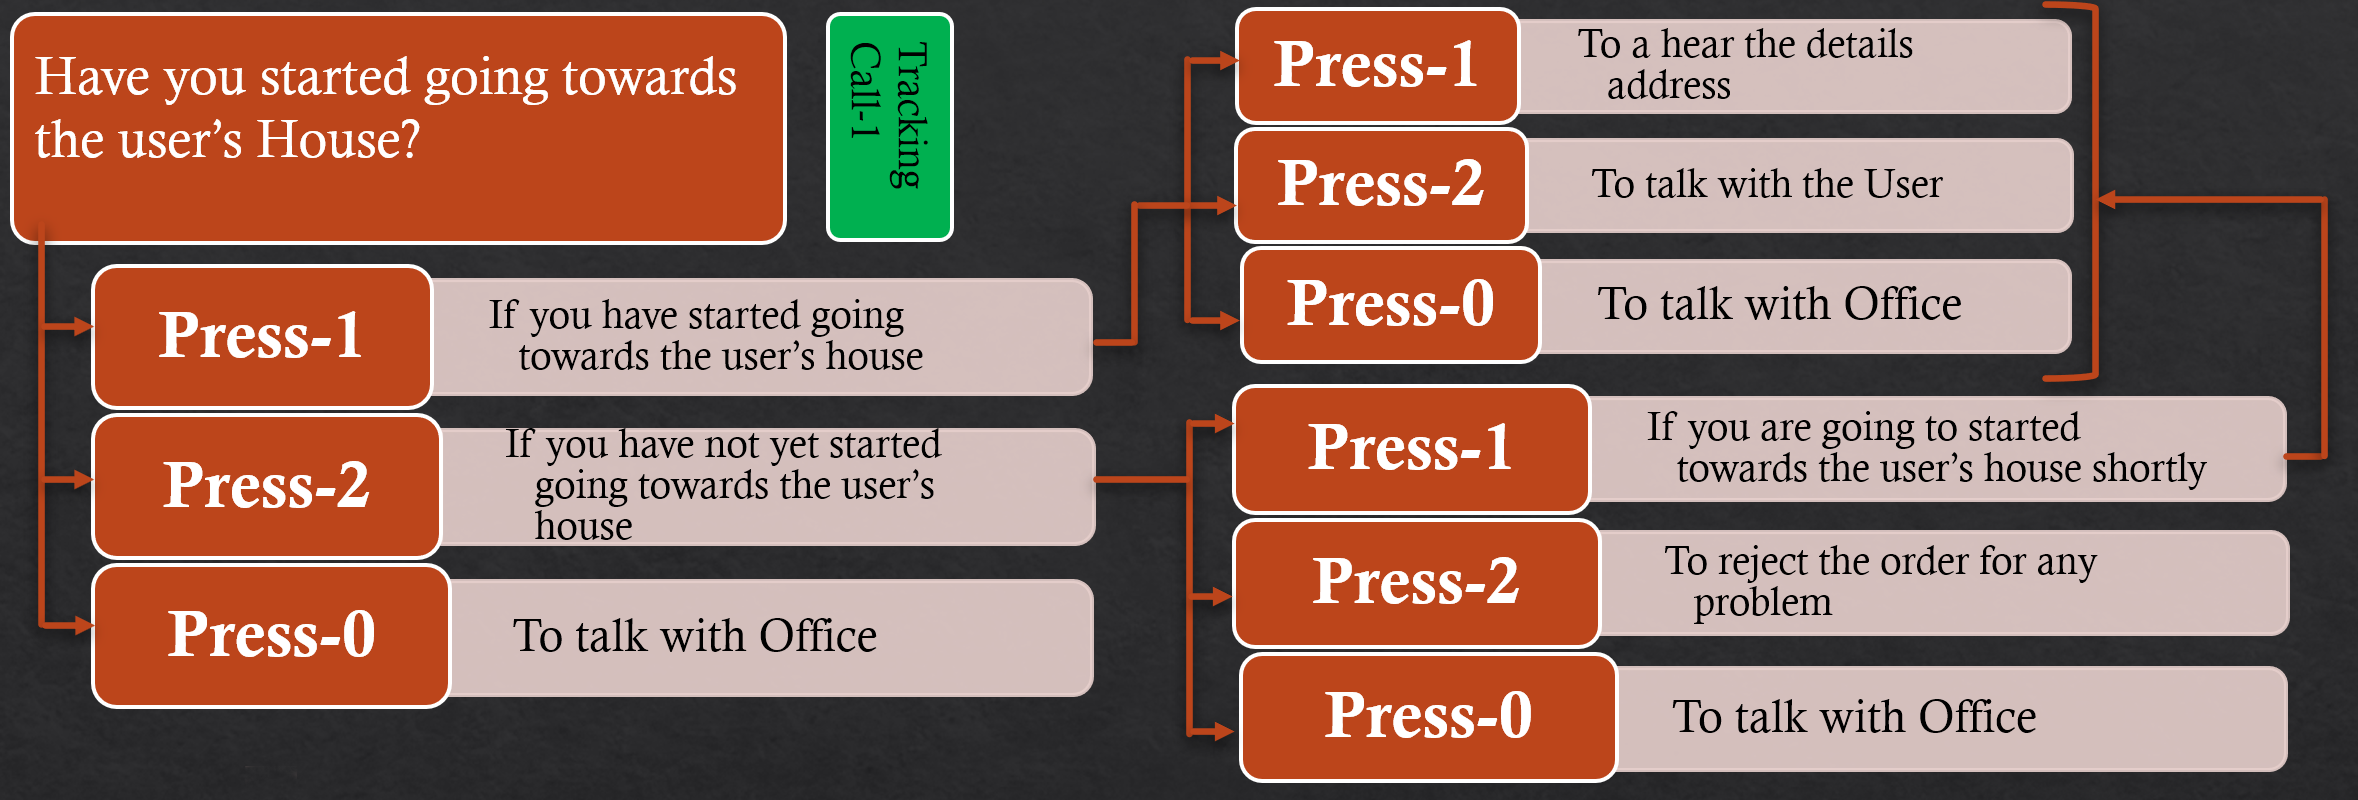
\includegraphics[width=1\linewidth]{images/ivrflow.png}
  \caption{The final design of one of the IVR menus, created by \PC{} in Microsoft Powerpoint.}\label{fig:ivrFlow}
  \Description{}
\end{figure}

This research focused on the \textit{design process} and how the values and priorities of each design partner was negotiated through the IVR design.  Data used in the analysis included: (i) recordings of workshop discussions that were transcribed; (ii) notes taken by researchers during workshops; and (iii) visual diagrams of the iterations of the IVR flow. 

Data analysis involved three iterative stages: (i) the final IVR flow design was analysed to identify the specific points in a job cycle that domestic workers interacted directly with the IVR system; (ii) workshop transcriptions and meeting notes were then read multiple times to identify dialogue that directly or indirectly informed how and why workers would interact with the IVR system at each point; (iii) finally, dialogue between each stakeholder was analysed thematically to identify the values, motivators and assumptions that were surfaced and negotiated through this design process to reveal that process behind the final IVR design. 
